\documentclass[11pt]{article}
\usepackage{amsmath,textcomp,amssymb,graphicx,alltt}
\usepackage[top=1in, bottom=1in, left=.5in, right=.5in]{geometry}

\def\Name{Allen Tang, Michelle Nguyen}  % Your name

\title{CS280 -- Spring 2015 -- Homework 2}
\author{\Name}
\markboth{CS280 -- Spring 2015 Homework 2 \Name}{CS174 -- Spring 2015 Homework 2 \Name}

\pagestyle{myheadings}
\begin{document}
\maketitle

\section*{1.1 Q1}
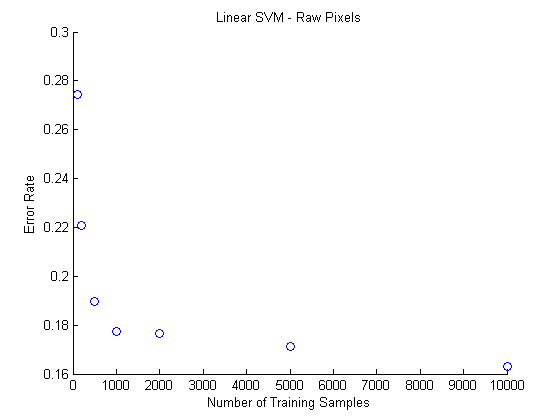
\includegraphics[scale=0.9]{diagrams/Question11.png}
\newpage
\section*{1.2 Q2}
\begin{itemize}
\item[a)]
Spatial pyramids give a regional "density" to the image. Some digits such as $4$ and $9$ may be classified similarly if we just use raw pixels, but if we use spatial pyramids, we are able to detect that many $4$'s have an opening on the top of the digit, where $9$'s do not. This difference can be captured by a spatial pyramid.
\item[b)]
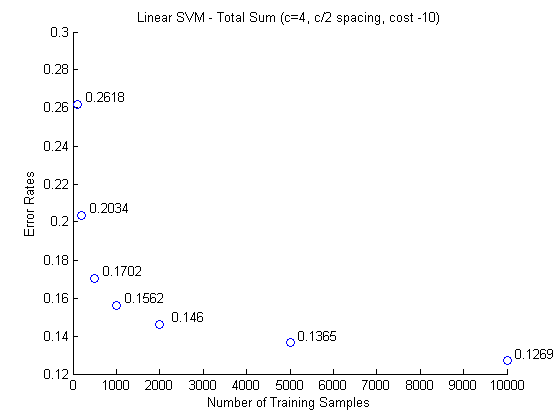
\includegraphics[scale=0.6]{diagrams/Question12b1.png}
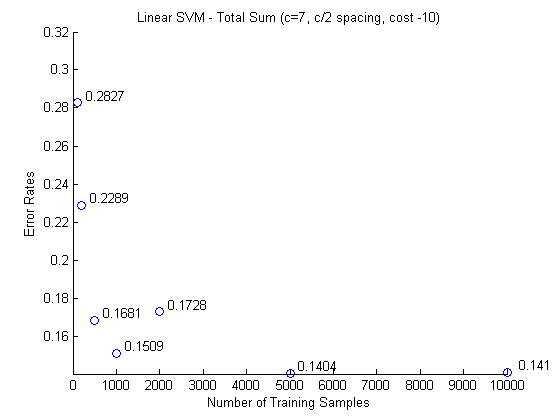
\includegraphics[scale=0.6]{diagrams/Question12b2.png}\\
We get roughly a $0.035\,(22\%)$ decrease on the 10,000 training sample set in error rate, which is significant.
\end{itemize}
\newpage


\newpage
\section*{1.3 Q3}
\pmb{Note: When comparing error rates, we chose the c (same across both trials) that obtains the lowest error rate.}	
\begin{itemize}
\item[a)]
Gradient orientations should help because they capture the relative ratios of gradient directions, which is invariant to slant (kind of like a shear).
\item[b)]
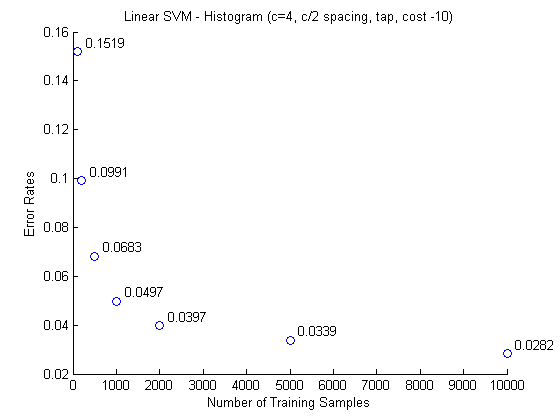
\includegraphics[scale=0.6]{diagrams/Question13b1.png}
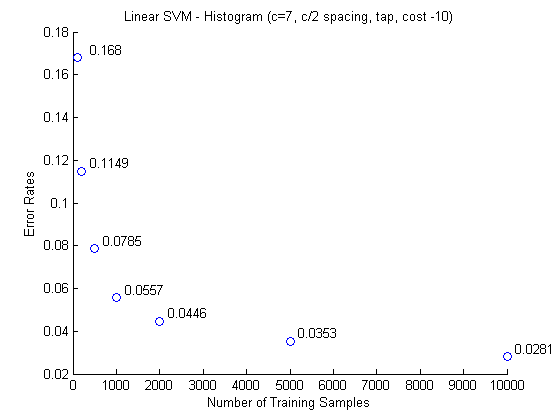
\includegraphics[scale=0.6]{diagrams/Question13b2.png}\\
We obtain a decrease in error rate of about $0.1\,(81\%)$ on the 10,000 training sample set, which is a tremendous increase in performance.
\item[c)]
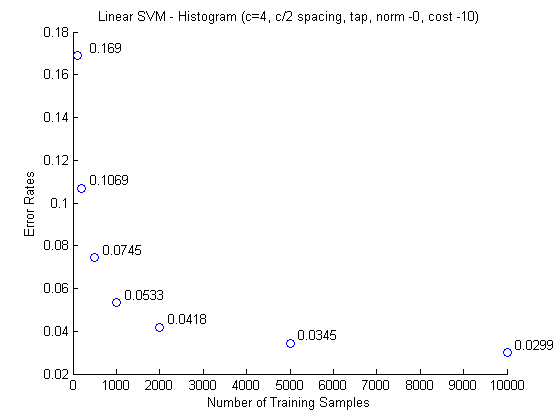
\includegraphics[scale=0.6]{diagrams/Question13c1.png}
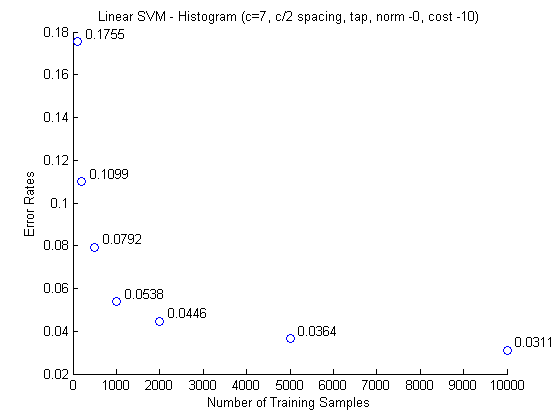
\includegraphics[scale=0.6]{diagrams/Question13c2.png}\\
The error rate drops by 0.017 on the 10,000 training sample set. Normalizing the histograms likely helps when considering two digits that are similar except for scaling. If we do not normalize the histograms, the gradient angles of the two digits would fall in the same bins but differ in magnitude. Normalizing the two histograms before making them features would make the features closer to each other. Since they have the same label, the probability that both are classified correctly may increase.
\item[d)]
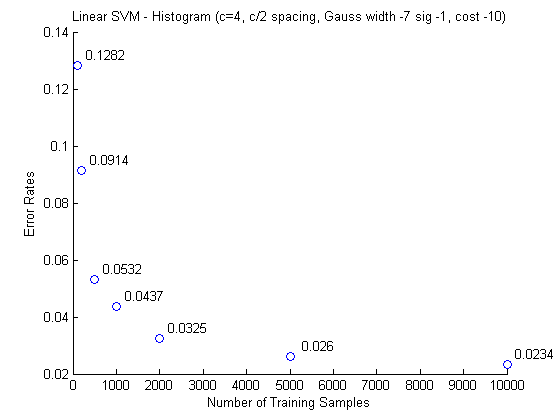
\includegraphics[scale=0.6]{diagrams/Question13d1.png}
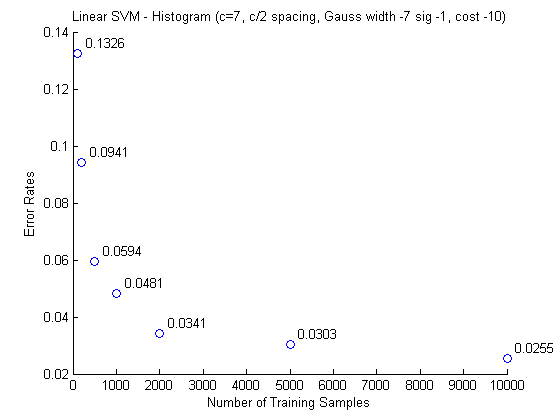
\includegraphics[scale=0.6]{diagrams/Question13d2.png}\\
The Gaussian derivative filter decreased the error rate by $0.0048\,(17\%)$ which is significant. The Gaussian derivative filter smooths out noise in the image and creates a cleaner gradient edge, which will certainly help binning, creating better features.
\item[e)]
The hyperparameter $c$ (cost) (SVM) required some adjustment. To choose an optimal $c$ that gives a good trade-off between generalizability and accuracy, we held out 10,000 examples from the training set and used it as cross-validation set, and ran different $c$ values, and decided a $c$ value of $10$ offered good performance.
\end{itemize}
\newpage
\section*{1.4}
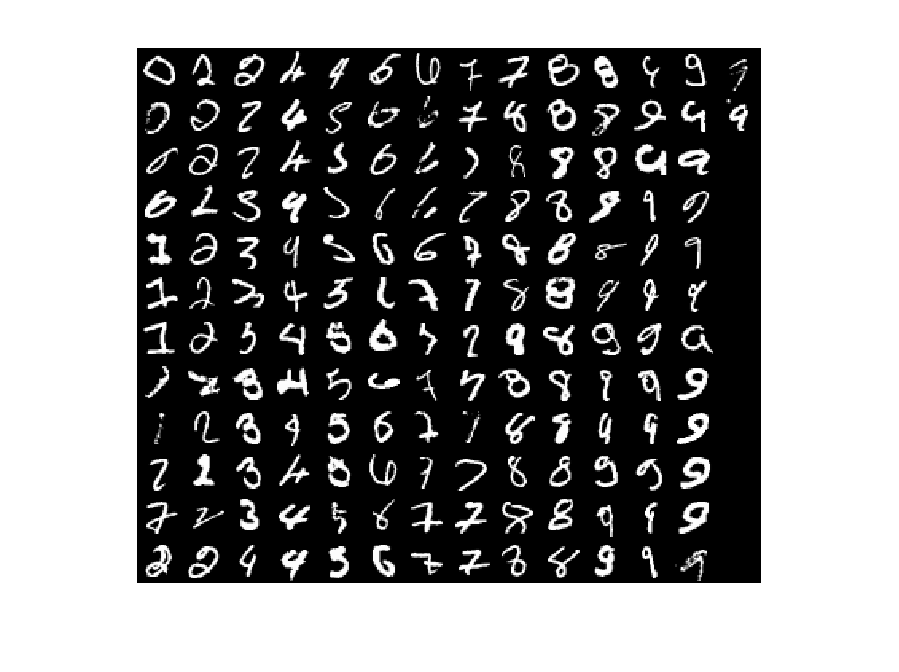
\includegraphics[scale=0.7]{diagrams/misclassifcation60k}\\
The errors on the classifier do seem pretty reasonable. About half of them seem to be ones that we can classify pretty quickly, but the other half are ones where we have to think a bit.
\newpage
\section*{1.6}
We ran orientation histograms with window size $4x4$ and obtained a 0.0158 error rate on the full training set.
\newpage
\section*{2.1.1}
\begin{itemize}
\item[1.] 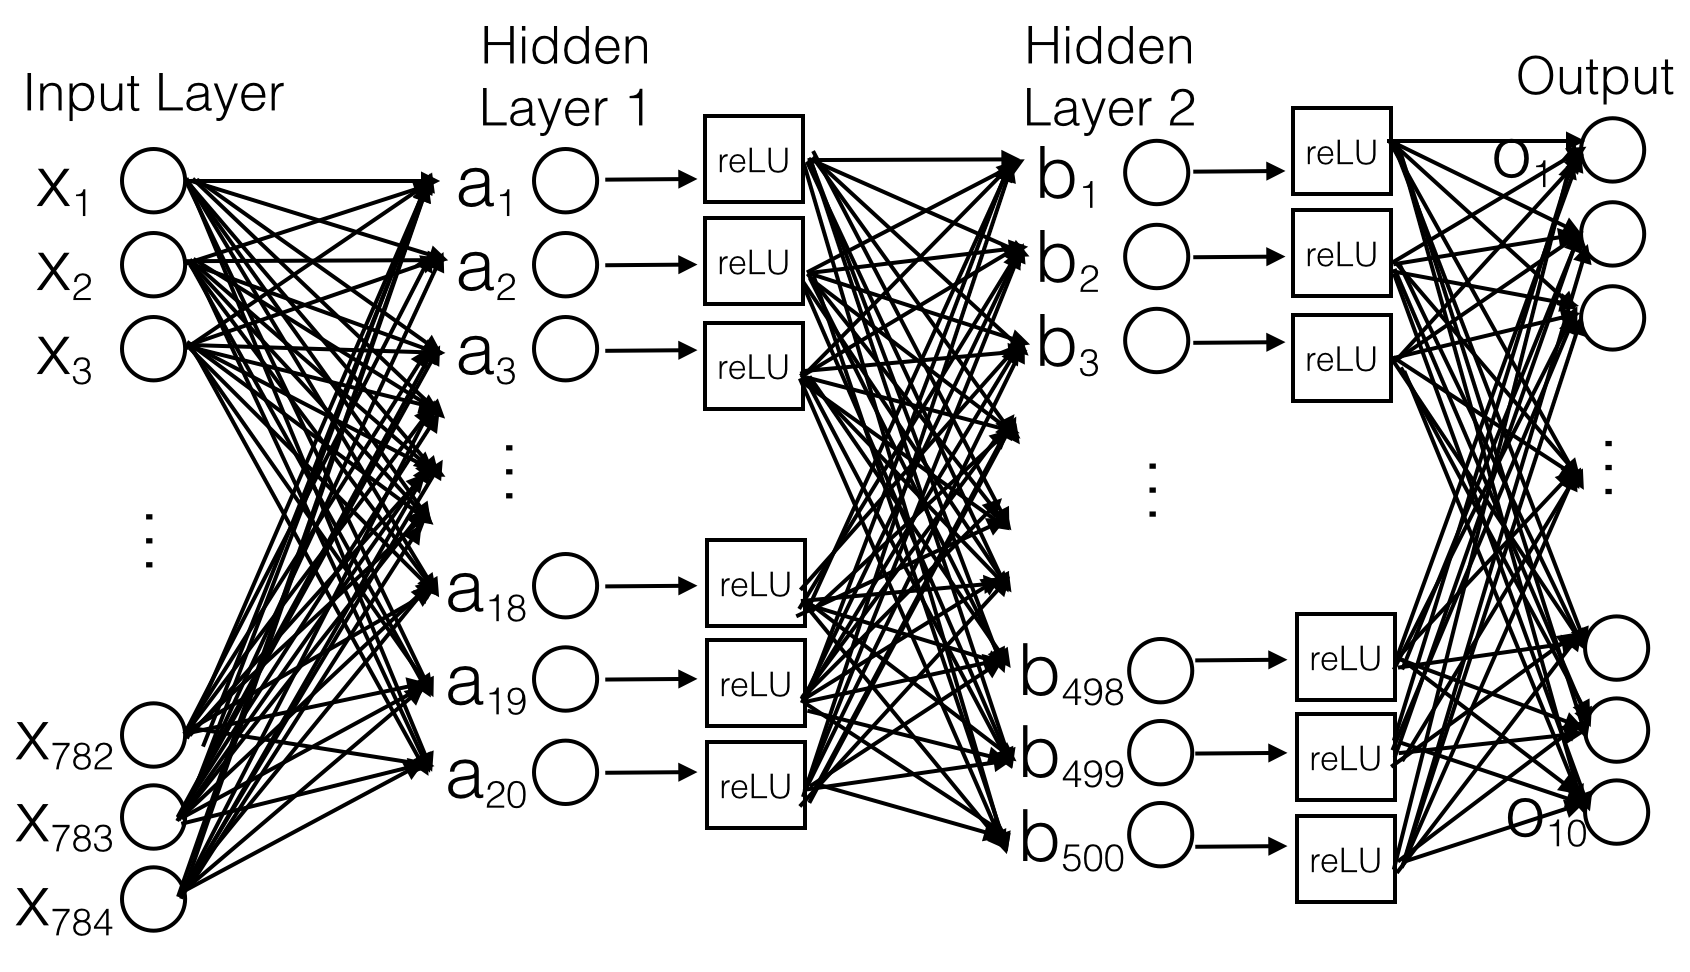
\includegraphics[scale=0.5]{diagrams/nnschematic.png}\\
\item[2.] Using a fully connected network of two hidden layers, we get an accuracy of 0.955156. This network has 4 params. Two of the params are the base learning rate and momentum which is specified in the solver. The other two parameters are the number of units per hidden layer for our two hidden layers. 
\item[3.] Using three hidden layers, we get an accuracy of 0.899219. This network has 5 params. As before, two of the params are for the base learning rate and momentum. Since we have three hidden layers, we have three parameters for the number of units for each of those layers.
\item[4.] We see that the accuracy is higher with two hidden layers than our network with three hidden layers. This is likely because the extra layer introduces more noise, and also because there is too much downsampling by having only 20 units in the first layer (as opposed to 500 units). 
\item[5.] We notice a decrease in accuracy when using a Sigmoid non-linearity. Besides an initial drop of loss after the first 100 iterations, there is little change in loss for the following iterations, whereas the loss with a reLU non-linearity steadily decreases. With two hidden layers and a Sigmoid non-linearity, we now get an accuracy of 0.884531. As the depth of the network increases, the gradient approaches 0 if a Sigmoid non-linearity is used. As a result, the larger the number of layers, the worse our accuracy becomes, which is undesirable. We see this by increasing the depth to three hidden layers, giving us an accuracy of 0.100313. ReLU non-linearities are much better because the gradients remain constant, which allows for faster learning and decreases the likelihood of the gradients becoming 0.

\end{itemize}
\newpage
\section*{2.2.1}
\begin{itemize}
\item[1.] Using the full training set with the given LeNet architecture, we get an accuracy of 0.988125. Using just 10K samples from the training set, the accuracy is 0.979062. The network has 7 params. Just as with the fully connected network, two of the params are the base learning rate and the momentum. Per convolution layer, of which we have two, we have two parameters: the number of units, and the kernel size. Finally, for our hidden inner product layer, we have one more parameter which is the number of units for that layer.
 Compared to the SVM classifier from part 1, our accuracy using 10K samples is a little under the best accuracy we got from part 1.
\item[2.] For 10K samples, our accuracy using LeNet is 0.979062 (also stated above), and our accuracy using a fully connected network of three layers is 0.899219, which is significantly worse.
\item[3.] Decreasing the number of units in our LeNet network, we get an accuracy of 0.97625, which is a slightly lower accuracy than when we had a larger number of units. This is still more than the accuracy for our fully connected network, because convolutional neural nets can handle cases of rotation, shift, and noise, much better than the fully connected network.
\item[4.] With a kernel size of 3, we get an accuracy of 0.976406. With a kernel size of 7, we get an accuracy of 0.97, which is slightly worse, but not much worse. 
\item[5.] 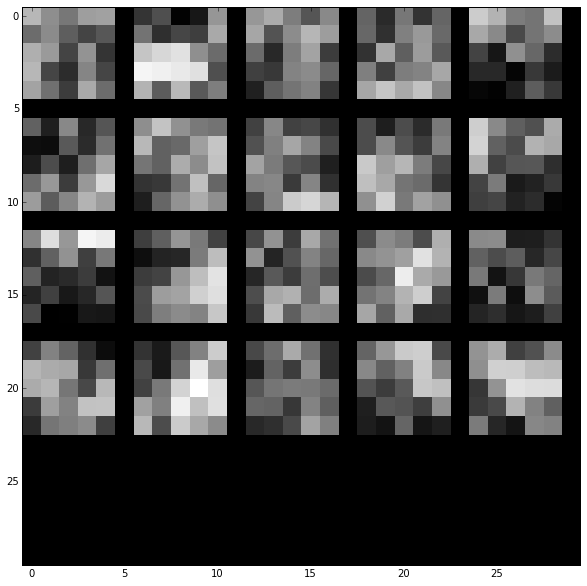
\includegraphics[scale=0.3]{diagrams/filter.png}\\
We see that our filter images show parts where there is a high contrast on one area of the square from another area of the square. For instance, there is no square that is completely white and no square that is completely black. From this, we can conclude that our first layer is finding features in the images where there are lines, edges, or corners. 
\item[6.] From our results, we can see that LeNet is much more accurate for the same number of hidden layers than a fully connected network is. However, most noticeably, the time it takes to train and test a fully connected network is faster than that of LeNet by about 10 times, for a performance that is not much worse than LeNet's. However, LeNet is fortified against variance in the dataset, such as rotations or translations, whereas fully connected networks are not. The LeNet architecture also has more params to consider, which would be much more time consuming to choose if we were to perform cross validation on our networks. The LeNet architecture is scalable to larger images because we can simply change the kernel size in the params, which would allow the filters to scale the image to smaller, more important parts.
\end{itemize}
\newpage
\section*{3}
We want to create a program that can detect various features from a person's headshot. For example, we want to be able to determine the shape of a person's face (round, long, oval, etc), their eye color, hair color, hair length, and so on. This would be a great application for dating websites, which would allow users to filter for potential matches based on their preferences of the given attributes. Using our application, these attributes could be generated from the user's uploaded photos. We also think current dating websites where users can upload photos and manually describe their appearance would be a great source of data and labels for the training process.
\end{document}